\documentclass[11pt]{article}

\usepackage[a4paper,margin=25mm]{geometry}
\usepackage{amsmath,amssymb}
\usepackage{booktabs}
\usepackage{graphicx}
\usepackage{microtype}
\usepackage[numbers,sort&compress]{natbib}
\usepackage[hidelinks]{hyperref}
\usepackage{xcolor}

\title{TopoDialogue: Visualising and Operationally Distinguishing\\
Recurrent Semantic Trajectories in Multi-Turn Dialogue}
\author{Ryoko Sakakibara\\Independent Researcher}
\date{First-draft audit: 14 August 2026}

\newcommand{\system}{\textsc{TopoDialogue}}
\newcommand{\code}[1]{\texttt{#1}}

\begin{document}
\maketitle

\begin{abstract}
Long human--AI conversations may return to a similar semantic region without
being exact textual repetitions. A return may be unproductive, may add detail or
abstraction, or may precede a move into a new region. These cases are difficult
to distinguish in a flat transcript. We present \system, an offline,
provenance-aware research instrument that represents a dialogue as a
time-indexed three-dimensional trajectory and assigns one of four operational
classes: closed loop, spiral revisit, escape, or open trajectory. The current
implementation uses explicit semantic-node annotations when available and a
declared lexical fallback otherwise. It provides deterministic hash-based
display co-ordinates, four selectable height mappings, recurrence and progress
scores, first-occurrence speaker provenance, and warnings for known display
artefacts. We define the complete Phase-1 procedure and evaluate it with six
authored synthetic cases whose expected structures are known by construction.
Both the Python reference implementation and the browser implementation match
all six declared class and recurrence-source labels; these are
specification-conformance tests, not an estimate of accuracy on natural
conversation. The study shows that recurrence, progress within a revisit, and
feature provenance can be made inspectable and reproducible. It does not show
that the display recovers a unique semantic manifold, infers mental state, or
improves dialogue outcomes. We report projection instability, lexical
approximation, monotonic-time, and speaker-drift failure modes and set out the
human-annotated evaluation needed next.
\end{abstract}

\section{Introduction}

A multi-turn dialogue is usually presented as an ordered list of utterances.
That representation preserves wording and order but makes recurrent structure
hard to inspect: a conversation can revisit a concern through paraphrase, return
to an assistant-supplied hypothesis after the user rejects it, or revisit a
topic while adding constraints and alternatives. Research on conversation
dynamics has shown that interactional change contains information not captured
by conventional topical summaries \citep{hua2024dynamics}. Other work has mapped
conversation turns into high-dimensional text representations to study topical
flow \citep{fischer2024trajectories}. In LLM settings, semantic-space models
have also been used to plan multi-turn responses \citep{chen2025scope}, while
controlled simulations show that models can become unreliable when a task is
spread over several turns \citep{laban2025lost}.

These findings motivate an instrument-level question rather than a broad claim
about cognition: \emph{can returns to a similar semantic region, and progress
within those returns, be represented as a reproducible trajectory with explicit
speaker provenance?} \system{} is a Phase-1 implementation of that question.
Its contribution is deliberately bounded:

\begin{enumerate}
  \item a fully specified, deterministic display co-ordinate system;
  \item operational definitions of revisit, progress, closed loop, spiral
        revisit, escape, and open trajectory;
  \item separate first-occurrence provenance for user- and assistant-originated
        features;
  \item six known synthetic cases, including adversarial display cases; and
  \item explicit reporting of conditions under which the geometry may mislead.
\end{enumerate}

The name \emph{TopoDialogue} comes from a broader design programme concerned
with preserving relational structure, simultaneity, contradiction, provenance,
embodiment, culture, privacy, and rendering control. This paper does not claim
to implement that programme in full. In particular, version 1 computes no
persistent homology, Betti number, or other topological invariant. Although
topological data analysis has an established and developing NLP literature
\citep{uchendu2026tda}, the present method is a geometric visual instrument with
rule-based operational labels. ``Topology'' is therefore design provenance,
not a mathematical result.

\section{Related work}

\paragraph{Conversation dynamics and trajectories.}
Hua et al. introduced summaries of conversation dynamics and evaluated their
utility in forecasting a later interactional outcome \citep{hua2024dynamics}.
Fischer and Ram represented dyadic conversations as trajectories derived from
text embeddings and quantified topical spread and alignment
\citep{fischer2024trajectories}. \system{} shares the premise that the route
through a conversation is worth inspecting, but it addresses a narrower
research-software problem: deterministic recurrence diagnostics for a single
transcript. It neither summarises interpersonal tone nor estimates personality.

\paragraph{Semantic-space dialogue models.}
SCOPE models stochastic transitions and rewards in a semantic space for
efficient conversation planning \citep{chen2025scope}. \system{} does not plan
responses or learn a transition model. It retrospectively displays turns and
applies declared recurrence rules. The distinction matters because a useful
plot does not by itself establish an effective intervention policy.

\paragraph{Recurrence and failure over repeated transformations.}
Wang et al. report periodic attractor cycles in successive LLM paraphrasing
\citep{wang2025attractor}. Their iterative paraphrase setting gives concrete
evidence that repeated model transformations can converge to periodic textual
states, but it is not evidence that ordinary human--LLM conversations obey the
same dynamics. Laban et al. report reduced reliability in simulated multi-turn
task completion relative to single-turn presentation \citep{laban2025lost}.
Together these studies justify examining recurrence and path dependence; they
do not validate the labels produced by \system{}.

\paragraph{Relation to topological data analysis.}
The NLP literature surveyed by Uchendu and Le includes methods that compute
geometric or topological descriptors from text representations
\citep{uchendu2026tda}. Version 1 of \system{} does not do so. Calling a visible
curve a ``loop'' or ``spiral'' is especially risky because projection alone can
create apparent curvature. Our class labels are consequently derived from
feature recurrence and progress rules, not from the rendered silhouette.

\section{Method}

\subsection{Input and feature provenance}

Let a dialogue contain turns $D=(u_1,\ldots,u_T)$. Each turn has a stable turn
identifier, a speaker in \{user, assistant, system\}, text, and optional semantic
annotations. The analyser selects one of three feature sources, in priority
order:

\begin{enumerate}
  \item explicit semantic-node keys, with optional confidence and abstraction;
  \item structured annotation fields such as frame, operator, state, and topic;
  \item case-folded word and character-trigram features as a lexical fallback.
\end{enumerate}

The resulting feature set for turn $t$ is $F_t$. The lexical fallback is not a
semantic embedding: it may miss paraphrases and overstate orthographic overlap.
Every report records the source used for each point and emits a warning whenever
the fallback is present.

For every feature $f$, origin $o(f)$ is the speaker of the first turn containing
$f$. New features at turn $t$ are
\begin{equation}
N_t = F_t \setminus \bigcup_{i<t}F_i.
\end{equation}
User- and assistant-originated novelty counts are obtained by grouping $N_t$ by
$o(f)$. This is a provenance rule, not a claim that the first speaker caused the
underlying idea.

\subsection{Deterministic display co-ordinates}

For each of three display components, every feature is mapped to a signed scalar
by a seeded FNV-1a hash. Scalars are averaged within the turn, mean-centred over
the dialogue, and scaled to $[-52,52]$. The first two components form semantic
projection $X$ and $Y$. The seed is stored in the report; the default is 1729.
This procedure makes the same input reproducible within an implementation, but
it does not recover a privileged psychological or linguistic axis.

The third co-ordinate is selectable:

\begin{description}
  \item[Time] maps turn order linearly to $[-50,50]$. Every non-trivial path
        rises, so height alone cannot indicate progress.
  \item[Revisit count] maps cumulative visits to an identical feature signature
        to $[-50,50]$.
  \item[Abstraction] maps an explicit annotation, or a declared node-type
        heuristic, from $[0,1]$ to $[-50,50]$. It is not psychological depth.
  \item[Alternative component] uses the third hash projection component for a
        display comparison.
\end{description}

Projection stability is a diagnostic rather than an inferential statistic. The
implementation repeats the two-dimensional projection with seed
$1729+104729$, computes all pairwise distances, and reports their Pearson
correlation clipped to $[0,1]$. Values below 0.65 trigger a seed-sensitivity
warning. A value of 1 for a degenerate arrangement should not be read as broad
robustness.

\subsection{Recurrence, progress, and LoopScore}

For turn $t$, the analyser searches up to 200 earlier turns, excluding the
immediately preceding turn by requiring a gap of at least two. Similarity to a
candidate anchor $j$ is Jaccard similarity,
\begin{equation}
s(t,j)=\frac{|F_t\cap F_j|}{|F_t\cup F_j|}.
\end{equation}
The best eligible anchor is $j_t=\arg\max_j s(t,j)$. Turn $t$ is a revisit when
$s(t,j_t)\geq 0.5$.

Let $a_t\in[0,1]$ be the operational abstraction value. Progress on a revisit is
\begin{equation}
p_t=\min\left(1,\;0.7\frac{|N_t|}{\max(1,|F_t|)}+
0.3\max(0,a_t-a_{j_t})\right).
\end{equation}
Non-revisits have $p_t=0$. For the set of revisits $R$, define
\begin{equation}
\overline{s}=\frac{1}{|R|}\sum_{t\in R}s(t,j_t),\qquad
\overline{p}=\frac{1}{|R|}\sum_{t\in R}p_t,
\end{equation}
and
\begin{equation}
\mathrm{LoopScore}=\operatorname{clip}_{[0,1]}\bigl(\overline{s}(1-\overline{p})\bigr).
\end{equation}
LoopScore is a descriptive software quantity. It is not a calibrated measure of
psychological state, conversational quality, or clinical risk.

\subsection{Operational classes}

Classification follows a fixed priority order:

\begin{enumerate}
  \item fewer than three turns: \emph{insufficient data};
  \item no revisits: \emph{open trajectory};
  \item an escape event: \emph{escape};
  \item mean revisit progress or mean positive abstraction gain at least 0.2:
        \emph{spiral revisit};
  \item otherwise: \emph{closed loop}.
\end{enumerate}

After each revisit, escape is true if, within the next five turns, there is a
user turn whose best similarity is below $0.5\times0.55=0.275$, which introduces
at least one new feature, and after which no further revisit occurs within the
remaining window. This rule explains why an escape case may retain a high
LoopScore: the score describes the preceding recurrent region, while the class
records the subsequent finite-window transition.

Recurrence source is computed from the speakers of revisit turns. More
assistant than user revisits gives \emph{assistant}; more user than assistant
gives \emph{user}; a tie gives \emph{mixed}; and no revisits gives \emph{none}.
This identifies where repeated features reappear. It does not establish causal
responsibility.

\section{Synthetic validation}

\subsection{Design}

Six six-turn fixtures were authored with explicit node keys and abstraction
values. Their expected labels follow directly from their construction:

\begin{enumerate}
  \item \emph{exact loop}: all turns share one feature;
  \item \emph{spiral revisit}: a shared garden feature accumulates soil and
        seasonal-change features while abstraction rises;
  \item \emph{open trajectory}: every turn occupies a distinct feature region;
  \item \emph{assistant-induced loop}: the assistant restores the same
        hypothesis after user turns introduce other regions;
  \item \emph{spiral escape}: a recurrent constraint is followed by a new
        user-originated action and desire region; and
  \item \emph{speaker drift}: user and assistant alternate between two separate
        recurrent branches, a stress case for visual interpretation.
\end{enumerate}

The manifest declares both expected shape and recurrence source. Tests execute
the Python reference implementation and the JavaScript browser implementation
against the same manifest. Reproducibility tests also compare repeated reports
under one seed and verify, on the spiral fixture, that changing the seed changes
display geometry without changing operational metrics other than the stability
diagnostic.

\subsection{Results}

Table~\ref{tab:synthetic} reports the Python reference results for
\code{trajectory-v1}, seed 1729. Both implementations matched all 12 declared
outputs (six class labels and six recurrence-source labels). This is exact
conformance on six constructed examples. It is not $100\%$ accuracy in a sampled
population and supplies no confidence interval for natural dialogue.

\begin{table*}[t]
\centering
\small
\caption{Synthetic Phase-1 results. $r$ is revisit rate, $\bar{s}$ mean revisit
similarity, $\bar{p}$ mean progress on revisit, $L$ LoopScore, $E$ Escape@5, and
$\rho$ projection stability.}
\label{tab:synthetic}
\begin{tabular}{llrrrrrr}
\toprule
Case & Class/source & $r$ & $\bar{s}$ & $\bar{p}$ & $L$ & $E$ & $\rho$ \\
\midrule
Exact loop & closed/mixed & .666667 & 1.000000 & .000000 & 1.000000 & No  & 1.000000 \\
Spiral revisit & spiral/mixed & .666667 & .583333 & .243333 & .441389 & No & .939956 \\
Open trajectory & open/none & .000000 & .000000 & .000000 & .000000 & No & .442795 \\
Assistant loop & closed/assistant & .333333 & 1.000000 & .000000 & 1.000000 & No & .434584 \\
Spiral escape & escape/mixed & .333333 & 1.000000 & .000000 & 1.000000 & Yes & .824146 \\
Speaker drift & closed/mixed & .666667 & 1.000000 & .000000 & 1.000000 & No & 1.000000 \\
\bottomrule
\end{tabular}
\end{table*}

The spiral-revisit case differs from the exact loop because its revisits add
features and increase the supplied abstraction value. The assistant-loop case
correctly assigns one novel hypothesis feature to the assistant and records two
assistant revisits versus no user revisits. The open and assistant-loop cases
trigger projection-sensitivity warnings because $\rho<0.65$. The escape fixture
illustrates the classifier's priority rule: it has a perfectly recurrent prefix
and hence LoopScore 1, yet its later user turn satisfies Escape@5.

\begin{figure*}[t]
\centering
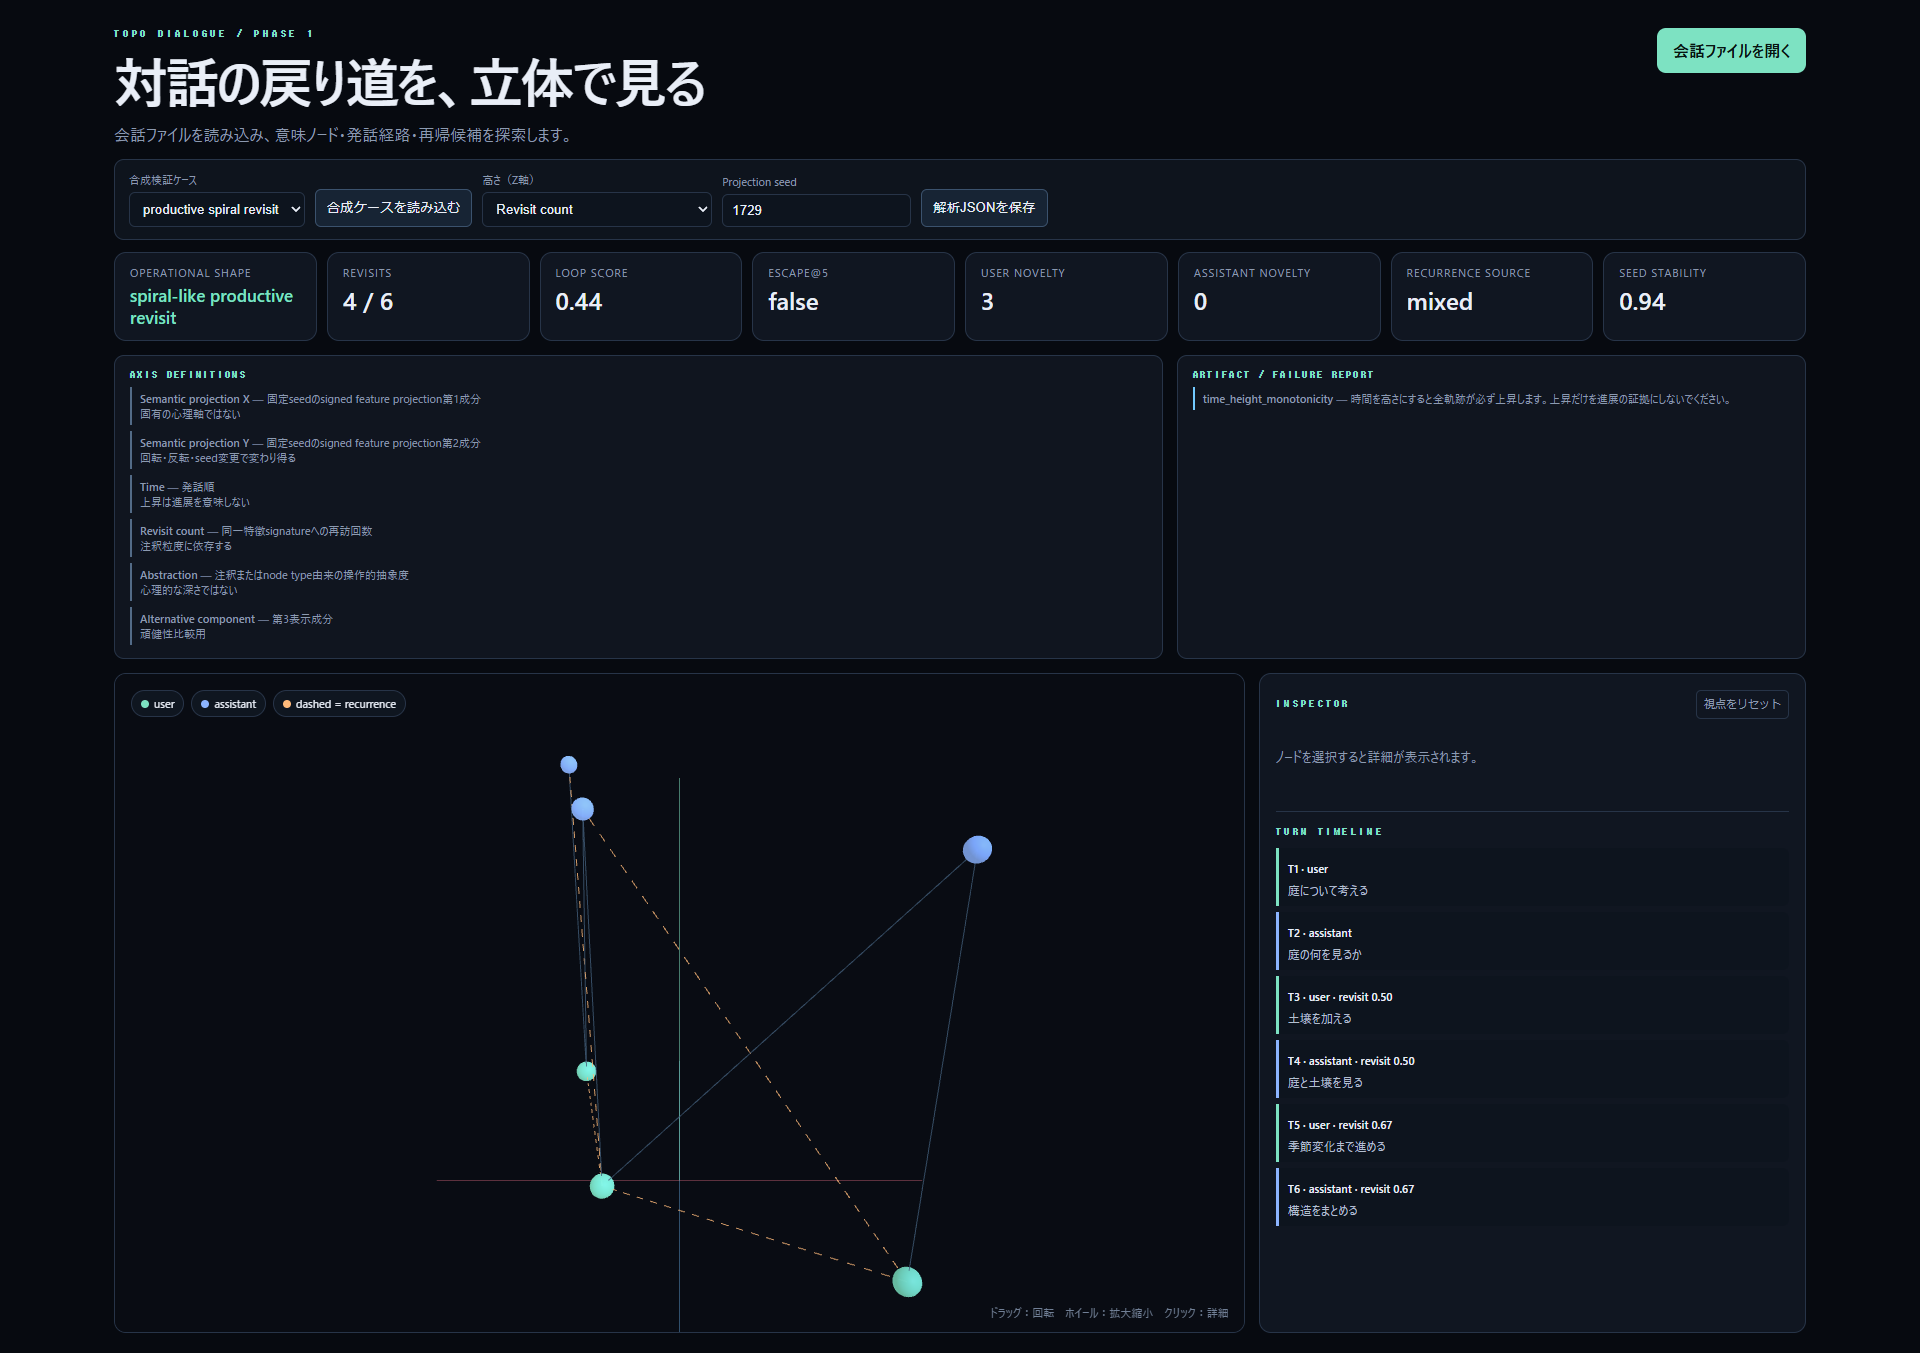
\includegraphics[width=.48\textwidth]{figures/fig01-spiral-revisit.png}\hfill
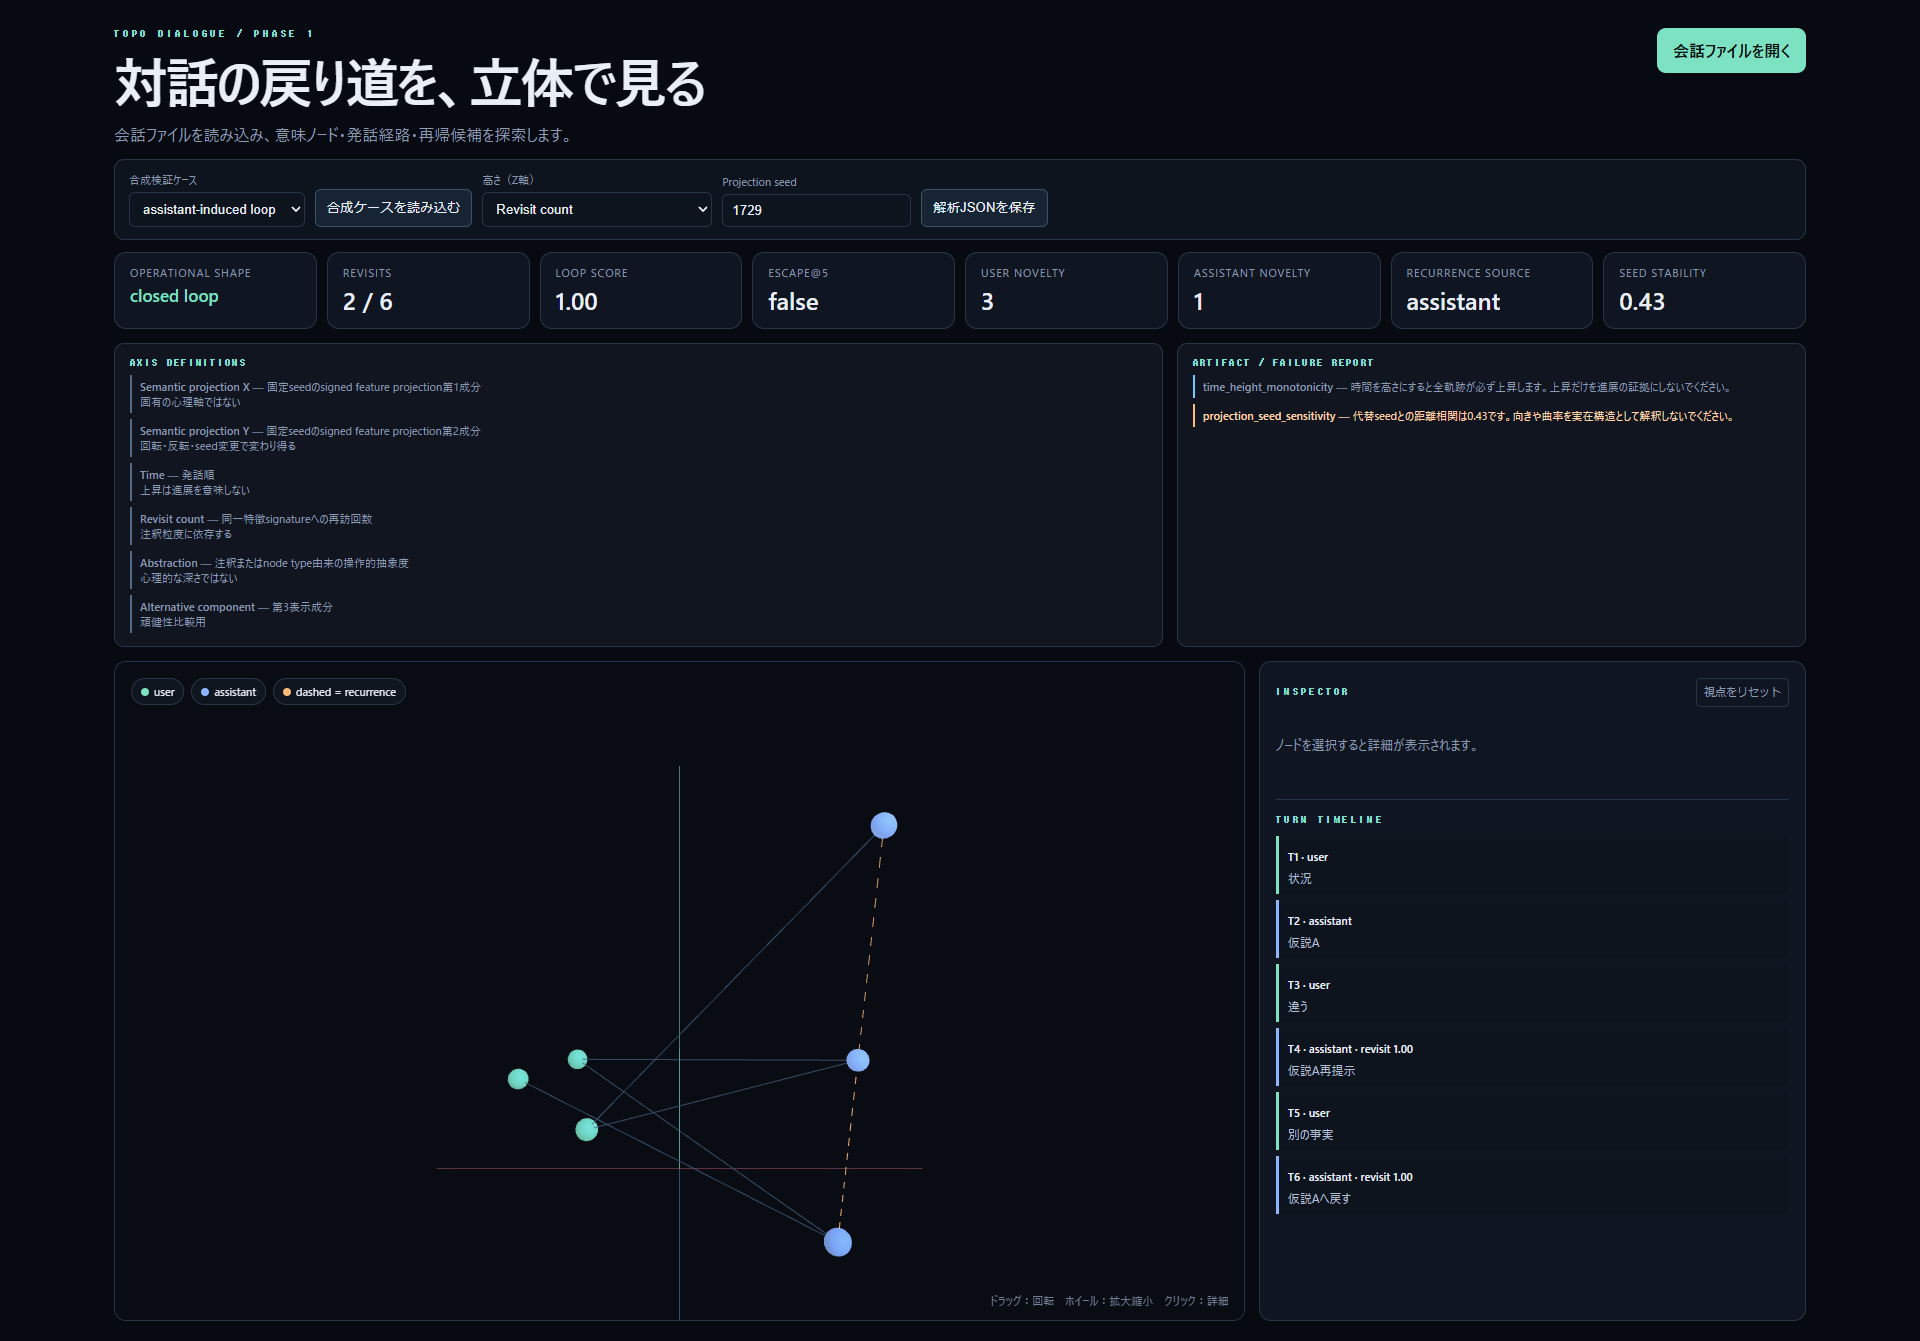
\includegraphics[width=.48\textwidth]{figures/fig02-assistant-induced-loop.png}
\caption{Left: the authored spiral-revisit fixture under the abstraction height
mapping. Right: assistant-induced recurrence. Shape labels come from the
feature-based rules, not visual curve recognition.}
\label{fig:spiral-assistant}
\end{figure*}

\begin{figure*}[t]
\centering
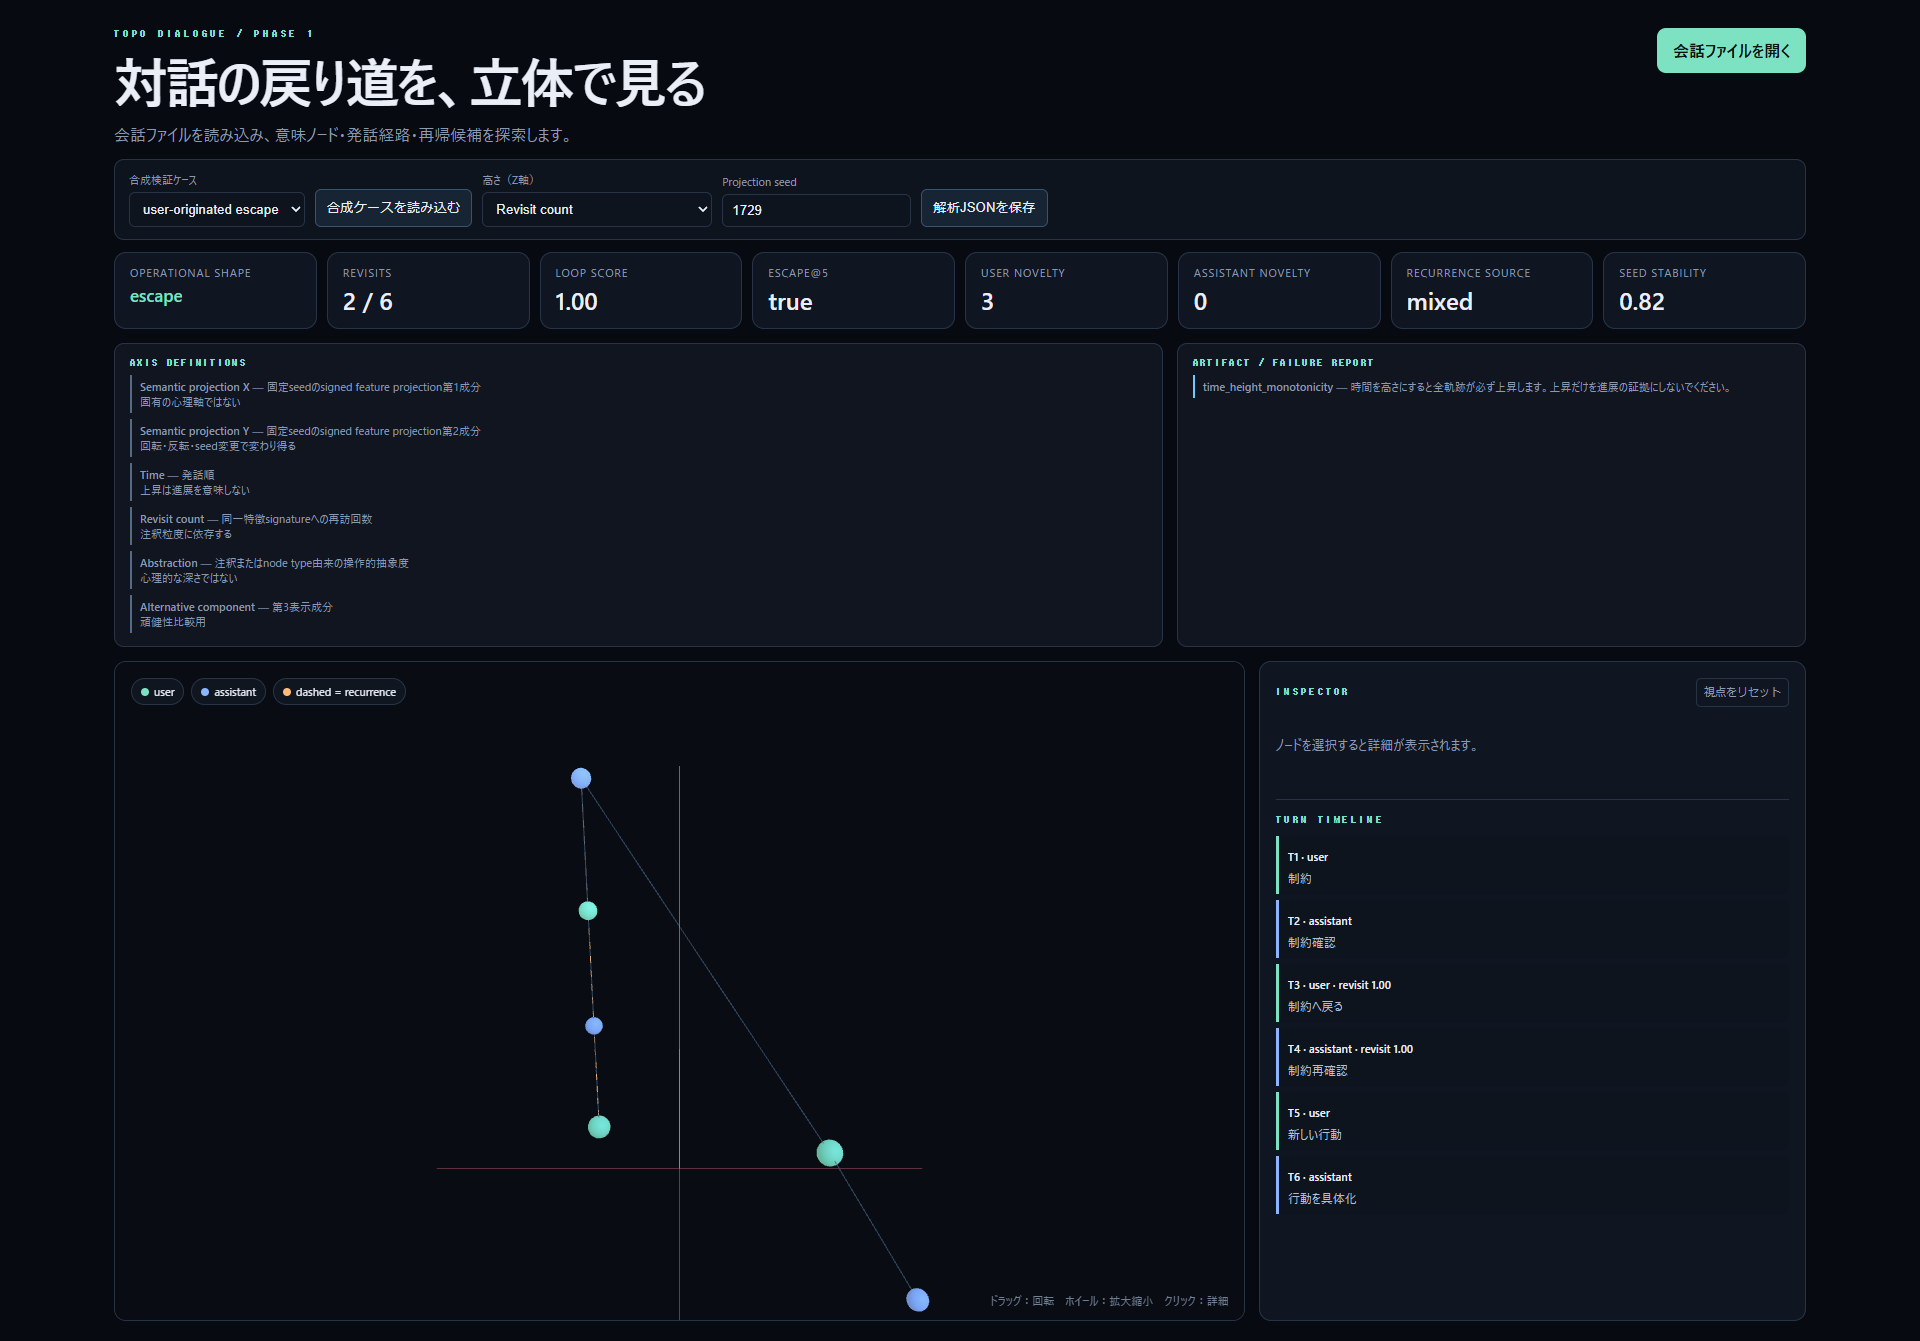
\includegraphics[width=.48\textwidth]{figures/fig03-user-originated-escape.png}\hfill
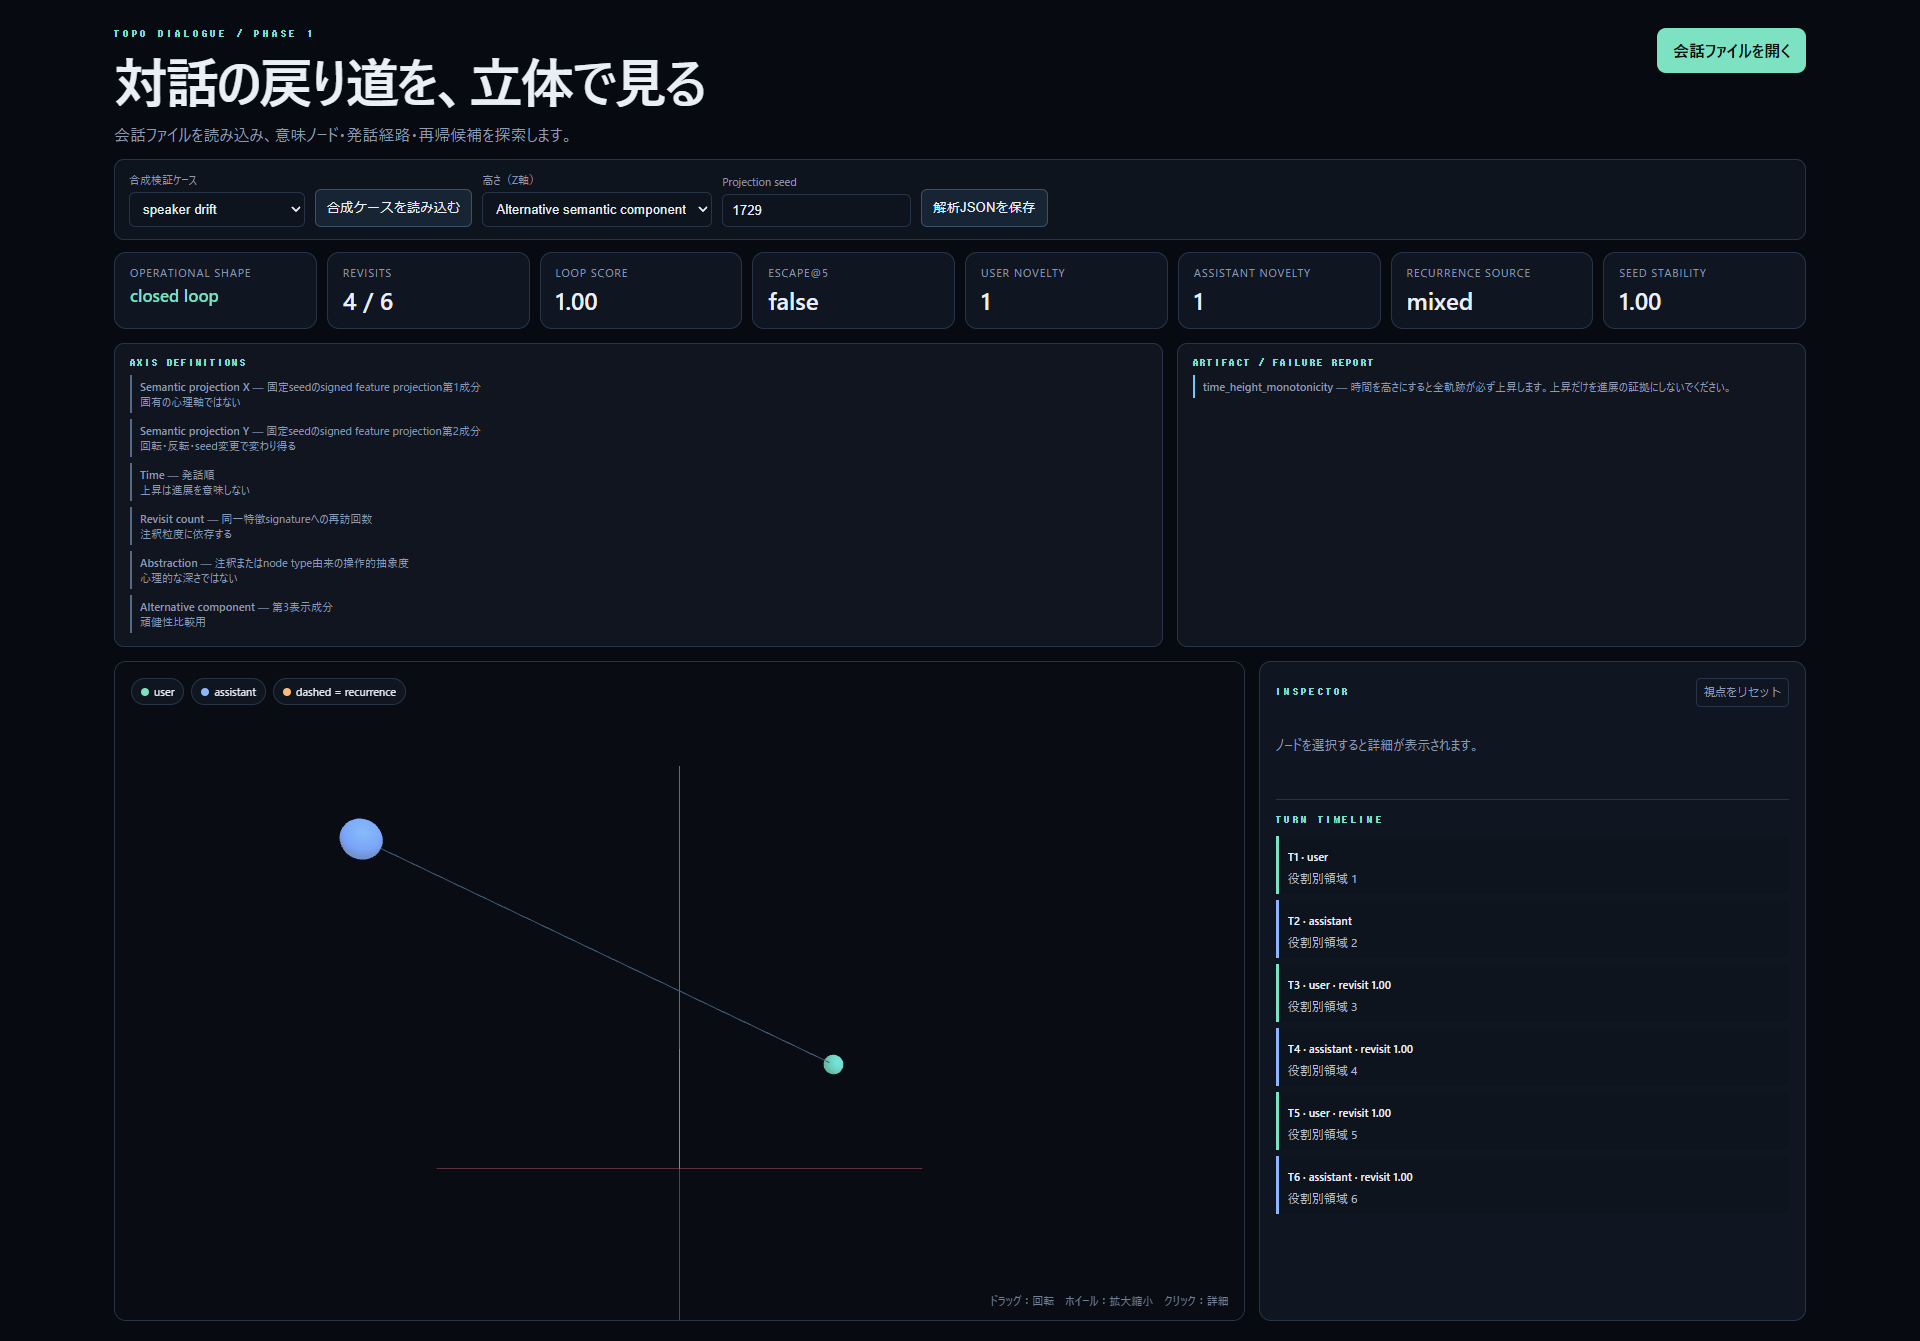
\includegraphics[width=.48\textwidth]{figures/fig04-speaker-drift-artifact.png}
\caption{Left: a recurrent constraint followed by an operational user escape.
Right: two speaker-conditioned branches rendered as one alternating path. The
right panel is an intentional visual stress case: a striking silhouette is not
evidence of a single shared semantic cycle.}
\label{fig:escape-drift}
\end{figure*}

\section{Artefacts and failure analysis}

\paragraph{Monotonic time.}
When time is used as height, every path rises from $-50$ to $50$. A helix-like
appearance can therefore be generated by the display convention. The software
always emits a monotonic-time notice, and the classifier never treats upward
motion alone as progress.

\paragraph{Lexical fallback.}
Unannotated exports use words and character trigrams. This is deterministic and
language-tolerant at the character level, but it is not robust to semantic
paraphrase. Reports disclose every fallback turn. A real-data evaluation must
compare lexical, embedding, and human annotation pipelines rather than merging
their results.

\paragraph{Seed sensitivity.}
Hash projections preserve no guarantee of neighbourhood fidelity. The
alternative-seed distance correlation exposes some instability, but one pair of
seeds cannot establish robustness. Consequently, orientation, handedness,
curvature, and apparent enclosure are not interpreted as real structure.

\paragraph{Speaker drift.}
The speaker-drift fixture alternates between a user region and a separate
assistant region. A single polyline visually connects them and can imply one
cycle. Speaker colour and point-level provenance partly expose the problem, but
the current implementation does not automatically warn when two role-specific
sub-trajectories collapse into one striking path.

\paragraph{Authored-fixture circularity.}
The fixtures and thresholds were designed together to test code paths. Their
agreement therefore demonstrates implementation consistency, not construct
validity. A further risk is that explicit node keys make recurrence easier than
it will be in natural text.

\paragraph{Runtime parity.}
Python and JavaScript share thresholds and fixture outcomes, but they do not
promise byte-identical reports across runtimes. Python uses a SHA-256 input hash;
the browser uses a shorter UI fingerprint, and Unicode token handling can differ.
Reproducibility claims in this paper are within-runtime and fixture-level unless
stated otherwise.

\section{Ethics, privacy, and intended use}

Dialogue logs may contain intimate, identifying, or third-party information.
The Phase-1 analyser runs locally and requires no network service, but local
execution alone does not provide consent, access control, retention limits, or
safe publication. Researchers should minimise collected text, preserve source
and speaker provenance, redact before sharing, document any annotation labour,
and avoid publishing raw personal conversations as examples.

\system{} is not a clinical, therapeutic, diagnostic, or risk-scoring tool. Its
terms ``loop'', ``progress'', and ``escape'' refer only to the equations and
finite-window rules in this paper. They must not be used to label a person as
stuck, recovered, insightful, resistant, or healthy. The display should support
inspection of a transcript, not replace reading it.

\section{Limitations and next evaluation}

The present evidence has five principal limits. First, six authored cases do
not establish external validity. Secondly, annotation keys are supplied rather
than inferred and may encode the expected answer. Thirdly, fixed hash
projections are display devices rather than modern semantic representations.
Fourthly, thresholds are design constants, not values estimated from labelled
data. Fifthly, the user/assistant origin rule records first appearance and cannot
resolve shared authorship, anticipation, quotation, or causal influence.

The next study should preregister an annotation protocol and use multiple human
annotators on held-out natural dialogues. It should measure inter-annotator
agreement for recurrence, productive revisit, and escape; compare lexical,
embedding, and annotated features; test multiple seeds and projection families;
report class-wise precision, recall, and calibration; and evaluate provenance
errors separately from shape errors. A blinded ablation should determine whether
three-dimensional views help analysts beyond a transcript, a similarity matrix,
and a two-dimensional timeline. Only after such evidence should transformation
operators or online intervention effects be evaluated.

\section{Conclusion}

\system{} translates the broad idea of preserving dialogue structure and
provenance into a small falsifiable instrument. Version 1 defines its axes,
reproduces a trajectory from fixed input and seed, distinguishes four
operational path classes, records first occurrence separately for user and
assistant features, and exposes several ways in which a compelling display can
mislead.
The six synthetic cases show that the software implements its declared rules.
They do not show that those rules describe natural conversations reliably. The
main result is therefore methodological: recurrence and change can be stated as
auditable operations before they are presented as shapes. That boundary makes a
subsequent empirical study possible without selling the shape itself as proof.

\section*{Language and reproducibility note}

The manuscript prose is written in British English. Paper titles in the
bibliography retain their published wording. Source code, synthetic fixtures,
tests, figure-capture scripts, and a claim audit are versioned together in the
project materials used for this draft. They are not yet deposited in a public
software archive; a public URL and archival identifier will be added in a
revision after an archival release.

\bibliographystyle{plainnat}
\bibliography{references}

\end{document}
